\documentclass[final,hyperref={pdfpagelabels=false}]{beamer}
\mode<presentation>
  {
  \usetheme{ntnuposter}
  }

\usepackage{amsmath,amsthm, amssymb, latexsym}
\boldmath
\usepackage[english]{babel}
\usepackage[latin1]{inputenc}
\usepackage[orientation=portrait,size=a0,scale=1.7,debug]{beamerposter}
\usepackage{ragged2e}

\setlength\parskip{1.5\baselineskip}

% Column support
\setlength{\columnsep}{8em}
\usepackage{multicol}

% Scale down from a0 to a4
\usepackage{pgfpages}
\pgfpagesuselayout{resize to}[a4paper]


\title[NTNU-poster]{Mal for EiT-poster i \LaTeX}
\author[Hove, Kvamsdal]{Per Kristian Hove og Trond Kvamsdal}
\institute[mia, NTNU]{mia: matematikk innen anvendelser, Eksperter i Team (V�ren 2011), NTNU}
\date{2010-04-28}


\begin{document}
  \begin{frame}{}
  \begin{columns}[t]
  \begin{column}{.97\textwidth}

	\justifying

    \begin{multicols}{2}
	{\Large Introduksjon}

    Lorem ipsum dolor sit amet, consectetur adipisicing
	elit, sed do eiusmod tempor incididunt ut labore et
	dolore magna aliqua. Ut enim ad minim veniam, quis
	nostrud exercitation ullamco laboris nisi ut aliquip
	ex ea $c = \lambda f$ commodo consequat. Duis aute irure dolor in
	reprehenderit in voluptate velit esse cillum dolore
	eu fugiat nulla pariatur. Excepteur sint occaecat
	cupidatat non proident, sunt in culpa qui officia
	deserunt mollit anim id est laborum:
	\[ \sin^{2}\theta_{hkl}=(\frac{\lambda^{2}}{4a^{2}})(h^{2}+k^{2}+l^{2}) \]



\vspace{1.0\baselineskip}
{\Large Hovedresultater}

	Lorem ipsum dolor sit amet, consectetur adipisicing
	elit, sed do eiusmod tempor incididunt ut labore et
	dolore magna aliqua. Ut enim ad minim veniam, quis
	nostrud exercitation ullamco laboris nisi ut aliquip
	ex ea commodo consequat. Duis aute irure dolor in
	reprehenderit in voluptate velit esse cillum dolore
	eu fugiat nulla pariatur. Excepteur sint occaecat
	cupidatat non proident, sunt in culpa qui officia
	deserunt mollit anim id est laborum.
	\begin{equation}
	\sin^{2}\theta_{i+1}-\sin^{2}\theta_{i}=(\frac{\lambda^{2}}{4a^{2}})\Delta n
	\end{equation}
	Lorem ipsum dolor sit amet, consectetur adipisicing
	elit, sed do eiusmod tempor incididunt ut labore et
	dolore magna aliqua. Ut enim ad minim veniam, quis
	nostrud exercitation ullamco laboris nisi ut aliquip
	ex ea commodo consequat. Duis aute irure dolor in
	reprehenderit in voluptate velit esse cillum dolore
	eu fugiat nulla pariatur. Excepteur sint occaecat
	cupidatat non proident, sunt in culpa qui officia
	deserunt mollit anim id est laborum.

    \vspace{1.0\baselineskip}	
	Lorem ipsum dolor sit amet, consectetur adipisicing
	elit, sed do eiusmod tempor incididunt ut labore et
	dolore magna aliqua. Ut enim ad minim veniam, quis
	nostrud exercitation ullamco laboris nisi ut aliquip
	ex ea $c = \lambda f$ commodo consequat:
	\[ \sin^{2}\theta_{hkl}=(\frac{\lambda^{2}}{4a^{2}})(h^{2}+k^{2}+l^{2}) \]
	Duis aute irure dolor in
	reprehenderit in voluptate velit esse cillum dolore
	eu fugiat nulla pariatur. Excepteur sint occaecat
	cupidatat non proident, sunt in culpa qui officia
	deserunt mollit anim id est laborum.
	Lorem ipsum dolor sit amet, consectetur adipisicing
	elit, sed do eiusmod tempor incididunt ut labore et
	dolore magna aliqua. Ut enim ad minim veniam, quis
	nostrud exercitation ullamco laboris nisi ut aliquip
	ex ea commodo consequat. Duis aute irure dolor in
	reprehenderit in voluptate velit esse cillum dolore
	eu fugiat nulla pariatur. Excepteur sint occaecat
	cupidatat non proident, sunt in culpa qui officia
	deserunt mollit anim id est laborum.
	\[ \sin^{2}\theta_{i+1}-\sin^{2}\theta_{i}=(\frac{\lambda^{2}}{4a^{2}})\Delta n \]
	Lorem ipsum dolor sit amet, consectetur adipisicing
	elit, sed do eiusmod tempor incididunt ut labore et
	dolore magna aliqua. Ut enim ad minim veniam, quis
	nostrud exercitation ullamco laboris nisi ut aliquip
	ex ea commodo consequat. Duis aute irure dolor in
	reprehenderit in voluptate velit esse cillum dolore
	eu fugiat nulla pariatur. Excepteur sint occaecat
	cupidatat non proident, sunt in culpa qui officia
	deserunt mollit anim id est laborum.

\vspace{1.0\baselineskip}
{\Large Konklusjoner}

    Duis aute irure dolor in
	reprehenderit in voluptate velit esse cillum dolore
	eu fugiat nulla pariatur. Excepteur sint occaecat
	cupidatat non proident, sunt in culpa qui officia
	deserunt mollit anim id est laborum.
	Lorem ipsum dolor sit amet, consectetur adipisicing
	elit, sed do eiusmod tempor incididunt ut labore et
	dolore magna aliqua. Ut enim ad minim veniam, quis
	nostrud exercitation ullamco laboris nisi ut aliquip
	ex ea commodo consequat. Duis aute irure dolor in
	reprehenderit in voluptate velit esse cillum dolore
	eu fugiat nulla pariatur. Excepteur sint occaecat
	cupidatat non proident, sunt in culpa qui officia
	deserunt mollit anim id est laborum.




    \begin{figure}
	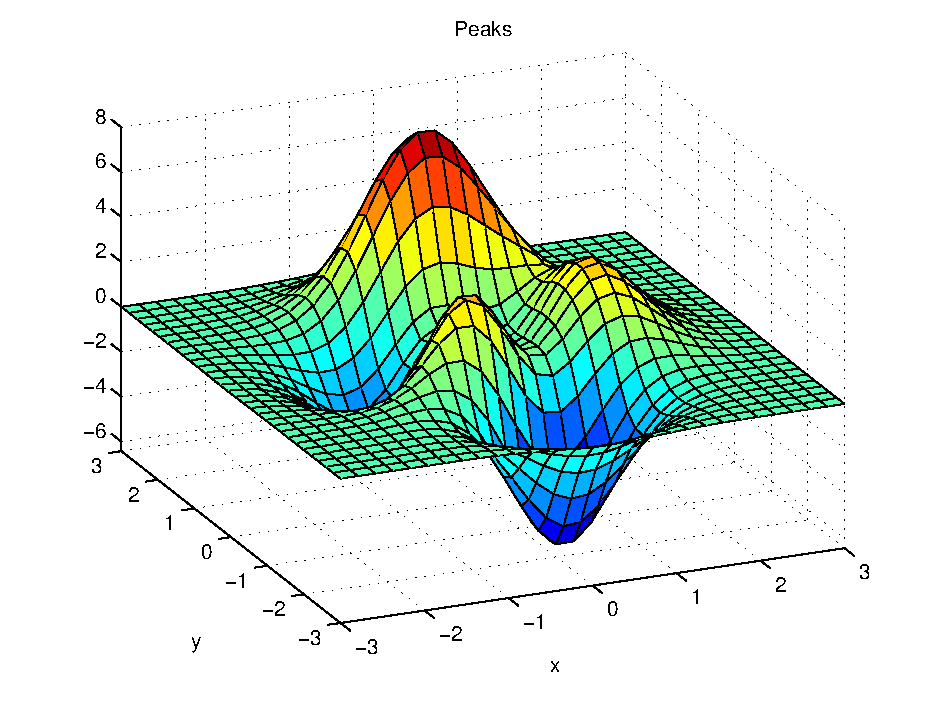
\includegraphics[width=\linewidth]{plot}
    \caption{Her viser vi resultater fra funskjonen $f_2(x,y)$}
    \end{figure}

    \end{multicols}



  \end{column}
  \end{columns}
  \end{frame}
\end{document}


%%%%%%%%%%%%%%%%%%%%%%%%%%%%%%%%%%%%%%%%%%%%%%%%%%%%%%%%%%%%%%%%%%%%%%%%%%%%%%%%%%%%%%%%%%%%%%%%%%%%
%%% Local Variables:
%%% mode: latex
%%% TeX-PDF-mode: t
%%% End:
